\documentclass[border=6pt]{standalone}
\usepackage{tikz}
\usetikzlibrary{arrows.meta,calc}
\begin{document}
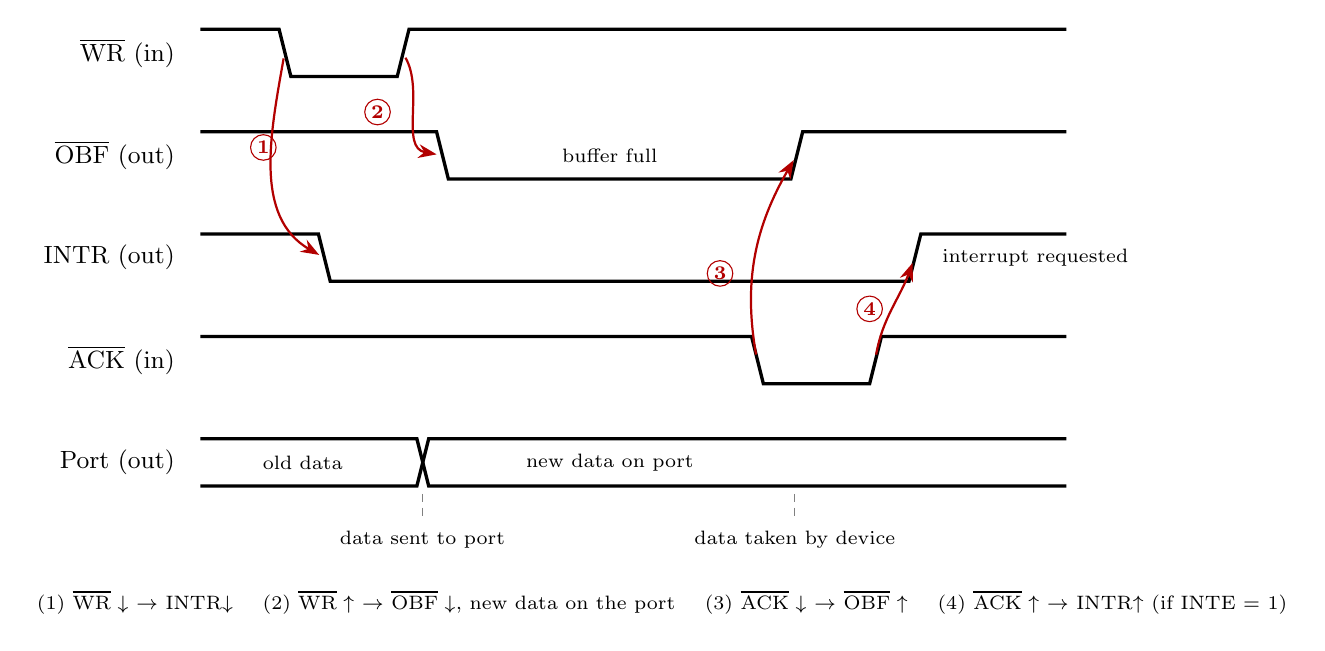
\begin{tikzpicture}[>=Stealth,font=\small,x=1cm,y=1cm,
 sig/.style={very thick},
 cause/.style={->,thick,red!70!black,shorten >=2pt,shorten <=2pt},
 num/.style={circle,draw,red!70!black,font=\scriptsize\bfseries,inner sep=1pt}]
\def\h{0.6}\def\e{0.15}
% rows: y of the low level
\def\yW{0}\def\yO{-1.3}\def\yI{-2.6}\def\yA{-3.9}\def\yP{-5.2}
\node[anchor=east] at (-0.2,\yW+0.3) {$\overline{\mathrm{WR}}$ (in)};
\node[anchor=east] at (-0.2,\yO+0.3) {$\overline{\mathrm{OBF}}$ (out)};
\node[anchor=east] at (-0.2,\yI+0.3) {INTR (out)};
\node[anchor=east] at (-0.2,\yA+0.3) {$\overline{\mathrm{ACK}}$ (in)};
\node[anchor=east] at (-0.2,\yP+0.3) {Port (out)};
% WR': low from 1 to 2.5
\draw[sig] (0,\yW+\h) -- (1,\yW+\h) -- (1+\e,\yW) -- (2.5,\yW) -- (2.5+\e,\yW+\h) -- (11,\yW+\h);
% OBF': falls after WR' rises (3.0), rises after ACK' falls (7.5)
\draw[sig] (0,\yO+\h) -- (3.0,\yO+\h) -- (3.0+\e,\yO) -- (7.5,\yO) -- (7.5+\e,\yO+\h) -- (11,\yO+\h);
\node[font=\scriptsize] at (5.2,\yO+0.3) {buffer full};
% INTR: falls after WR' falls (1.5), rises after ACK' rises (9.0)
\draw[sig] (0,\yI+\h) -- (1.5,\yI+\h) -- (1.5+\e,\yI) -- (9.0,\yI) -- (9.0+\e,\yI+\h) -- (11,\yI+\h);
\node[font=\scriptsize,anchor=west] at (9.3,\yI+0.3) {interrupt requested};
% ACK': low from 7 to 8.5
\draw[sig] (0,\yA+\h) -- (7.0,\yA+\h) -- (7.0+\e,\yA) -- (8.5,\yA) -- (8.5+\e,\yA+\h) -- (11,\yA+\h);
% Port: new data valid after WR' rises
\draw[sig] (0,\yP+\h) -- (2.75,\yP+\h) -- (2.9,\yP) -- (11,\yP);
\draw[sig] (0,\yP) -- (2.75,\yP) -- (2.9,\yP+\h) -- (11,\yP+\h);
\node[font=\scriptsize,fill=white,inner sep=1pt] at (1.3,\yP+0.3) {old data};
\node[font=\scriptsize,fill=white,inner sep=1pt] at (5.2,\yP+0.3) {new data on port};
\draw[gray,densely dashed] (2.82,\yP-0.1) -- (2.82,\yP-0.45) node[below,font=\scriptsize,black]{data sent to port};
\draw[gray,densely dashed] (7.55,\yP-0.1) -- (7.55,\yP-0.45) node[below,font=\scriptsize,black,align=center]{data taken by device};
% cause -> effect arrows
\draw[cause] (1.07,\yW+0.3) to[out=-100,in=150] (1.57,\yI+0.3);
\node[num] at (0.8,\yW-0.9) {1};
\draw[cause] (2.57,\yW+0.3) to[out=-60,in=170] (3.07,\yO+0.3);
\node[num] at (2.25,\yW-0.45) {2};
\draw[cause] (7.07,\yA+0.3) to[out=100,in=-120] (7.57,\yO+0.3);
\node[num] at (6.6,\yA+1.4) {3};
\draw[cause] (8.57,\yA+0.3) to[out=80,in=-110] (9.07,\yI+0.3);
\node[num] at (8.5,\yA+0.95) {4};
\node[font=\scriptsize,align=left,anchor=north west] at (-2.2,\yP-1.2) {%
(1) $\overline{\mathrm{WR}}\downarrow$ $\to$ INTR$\downarrow$ \quad
(2) $\overline{\mathrm{WR}}\uparrow$ $\to$ $\overline{\mathrm{OBF}}\downarrow$, new data on the port \quad
(3) $\overline{\mathrm{ACK}}\downarrow$ $\to$ $\overline{\mathrm{OBF}}\uparrow$ \quad
(4) $\overline{\mathrm{ACK}}\uparrow$ $\to$ INTR$\uparrow$ (if INTE = 1)};
\end{tikzpicture}
\end{document}
